

\tikzset{every picture/.style={line width=0.75pt}} %set default line width to 0.75pt        

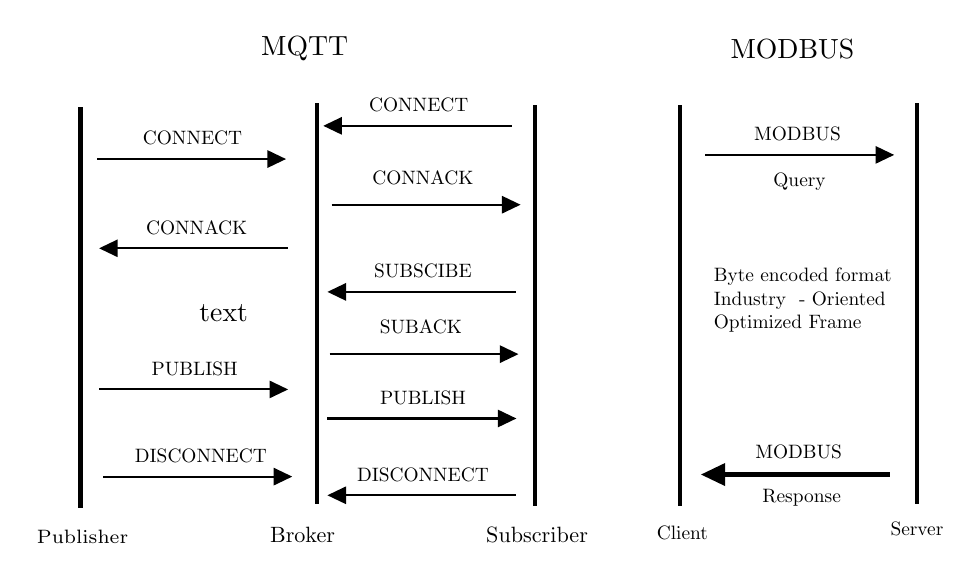
\begin{tikzpicture}[x=0.75pt,y=0.75pt,yscale=-1,xscale=1]
%uncomment if require: \path (0,300); %set diagram left start at 0, and has height of 300

%Straight Lines [id:da12798558333744703] 
\draw [line width=1.5]    (51,51) -- (51,244) ;


%Straight Lines [id:da11517902673265334] 
\draw [line width=1.5]    (165,49) -- (165,242) ;


%Straight Lines [id:da27778345517546654] 
\draw [line width=1.5]    (270,50) -- (270,243) ;


%Straight Lines [id:da4784433104779049] 
\draw [line width=1.5]    (340,50) -- (340,243) ;


%Straight Lines [id:da14318622021376104] 
\draw [line width=1.5]    (454,49) -- (454,242) ;


%Straight Lines [id:da2521307853666861] 
\draw [color={rgb, 255:red, 0; green, 0; blue, 0 }  ,draw opacity=1 ][line width=0.75]    (59,76) -- (148,76) ;
\draw [shift={(150,76)}, rotate = 180] [fill={rgb, 255:red, 0; green, 0; blue, 0 }  ,fill opacity=1 ][line width=0.75]  [draw opacity=0] (8.93,-4.29) -- (0,0) -- (8.93,4.29) -- cycle    ;

%Straight Lines [id:da416495389819703] 
\draw [color={rgb, 255:red, 0; green, 0; blue, 0 }  ,draw opacity=1 ][line width=0.75]    (62,119) -- (151,119) ;

\draw [shift={(60,119)}, rotate = 0] [fill={rgb, 255:red, 0; green, 0; blue, 0 }  ,fill opacity=1 ][line width=0.75]  [draw opacity=0] (8.93,-4.29) -- (0,0) -- (8.93,4.29) -- cycle    ;
%Straight Lines [id:da9635625455331085] 
\draw [color={rgb, 255:red, 0; green, 0; blue, 0 }  ,draw opacity=1 ][line width=0.75]    (60,187) -- (149,187) ;
\draw [shift={(151,187)}, rotate = 180] [fill={rgb, 255:red, 0; green, 0; blue, 0 }  ,fill opacity=1 ][line width=0.75]  [draw opacity=0] (8.93,-4.29) -- (0,0) -- (8.93,4.29) -- cycle    ;

%Straight Lines [id:da1895725774033723] 
\draw [color={rgb, 255:red, 0; green, 0; blue, 0 }  ,draw opacity=1 ][line width=0.75]    (62,229) -- (151,229) ;
\draw [shift={(153,229)}, rotate = 180] [fill={rgb, 255:red, 0; green, 0; blue, 0 }  ,fill opacity=1 ][line width=0.75]  [draw opacity=0] (8.93,-4.29) -- (0,0) -- (8.93,4.29) -- cycle    ;

%Straight Lines [id:da7272521685262943] 
\draw [color={rgb, 255:red, 0; green, 0; blue, 0 }  ,draw opacity=1 ][line width=0.75]    (170,60) -- (259,60) ;

\draw [shift={(168,60)}, rotate = 0] [fill={rgb, 255:red, 0; green, 0; blue, 0 }  ,fill opacity=1 ][line width=0.75]  [draw opacity=0] (8.93,-4.29) -- (0,0) -- (8.93,4.29) -- cycle    ;
%Straight Lines [id:da30340216601848824] 
\draw [color={rgb, 255:red, 0; green, 0; blue, 0 }  ,draw opacity=1 ][line width=0.75]    (172,98) -- (261,98) ;
\draw [shift={(263,98)}, rotate = 180] [fill={rgb, 255:red, 0; green, 0; blue, 0 }  ,fill opacity=1 ][line width=0.75]  [draw opacity=0] (8.93,-4.29) -- (0,0) -- (8.93,4.29) -- cycle    ;

%Straight Lines [id:da5689262114397526] 
\draw [color={rgb, 255:red, 0; green, 0; blue, 0 }  ,draw opacity=1 ][line width=0.75]    (172,140) -- (261,140) ;

\draw [shift={(170,140)}, rotate = 0] [fill={rgb, 255:red, 0; green, 0; blue, 0 }  ,fill opacity=1 ][line width=0.75]  [draw opacity=0] (8.93,-4.29) -- (0,0) -- (8.93,4.29) -- cycle    ;
%Straight Lines [id:da43739445383533293] 
\draw [color={rgb, 255:red, 0; green, 0; blue, 0 }  ,draw opacity=1 ][line width=0.75]    (171,170) -- (260,170) ;
\draw [shift={(262,170)}, rotate = 180] [fill={rgb, 255:red, 0; green, 0; blue, 0 }  ,fill opacity=1 ][line width=0.75]  [draw opacity=0] (8.93,-4.29) -- (0,0) -- (8.93,4.29) -- cycle    ;

%Straight Lines [id:da4265213474229044] 
\draw [color={rgb, 255:red, 0; green, 0; blue, 0 }  ,draw opacity=1 ][line width=0.75]    (170,201) -- (259,201) ;
\draw [shift={(261,201)}, rotate = 180] [fill={rgb, 255:red, 0; green, 0; blue, 0 }  ,fill opacity=1 ][line width=0.75]  [draw opacity=0] (8.93,-4.29) -- (0,0) -- (8.93,4.29) -- cycle    ;

%Straight Lines [id:da2890367081898375] 
\draw [color={rgb, 255:red, 0; green, 0; blue, 0 }  ,draw opacity=1 ][line width=0.75]    (172,238) -- (261,238) ;

\draw [shift={(170,238)}, rotate = 0] [fill={rgb, 255:red, 0; green, 0; blue, 0 }  ,fill opacity=1 ][line width=0.75]  [draw opacity=0] (8.93,-4.29) -- (0,0) -- (8.93,4.29) -- cycle    ;
%Straight Lines [id:da5478425871587402] 
\draw [color={rgb, 255:red, 0; green, 0; blue, 0 }  ,draw opacity=1 ][line width=0.75]    (352,74) -- (441,74) ;
\draw [shift={(443,74)}, rotate = 180] [fill={rgb, 255:red, 0; green, 0; blue, 0 }  ,fill opacity=1 ][line width=0.75]  [draw opacity=0] (8.93,-4.29) -- (0,0) -- (8.93,4.29) -- cycle    ;

%Straight Lines [id:da6706223138763108] 
\draw [color={rgb, 255:red, 0; green, 0; blue, 0 }  ,draw opacity=1 ][line width=1.5]    (353,228) -- (441,228) ;

\draw [shift={(350,228)}, rotate = 0] [fill={rgb, 255:red, 0; green, 0; blue, 0 }  ,fill opacity=1 ][line width=1.5]  [draw opacity=0] (11.61,-5.58) -- (0,0) -- (11.61,5.58) -- cycle    ;

% Text Node
\draw (159,23) node  [align=left] {MQTT};
% Text Node
\draw (394,23) node  [align=left] {MODBUS};
% Text Node
\draw (52,258) node  [align=left] {{\scriptsize Publisher}};
% Text Node
\draw (158,257) node [scale=0.8] [align=left] {Broker};
% Text Node
\draw (271,257) node [scale=0.8] [align=left] {Subscriber};
% Text Node
\draw (105,66) node [scale=0.7] [align=left] {CONNECT};
% Text Node
\draw (107,109) node [scale=0.7] [align=left] {CONNACK};
% Text Node
\draw (106,177) node [scale=0.7] [align=left] {PUBLISH};
% Text Node
\draw (109,219) node [scale=0.7] [align=left] {DISCONNECT};
% Text Node
\draw (214,50) node [scale=0.7] [align=left] {CONNECT};
% Text Node
\draw (216,85) node [scale=0.7] [align=left] {CONNACK};
% Text Node
\draw (216,130) node [scale=0.7] [align=left] {SUBSCIBE};
% Text Node
\draw (215,157) node [scale=0.7] [align=left] {SUBACK};
% Text Node
\draw (216,191) node [scale=0.7] [align=left] {PUBLISH};
% Text Node
\draw (216,228) node [scale=0.7] [align=left] {DISCONNECT};
% Text Node
\draw (398,64) node [scale=0.7] [align=left] {MODBUS };
% Text Node
\draw (399,87) node [scale=0.7] [align=left] {Query };
% Text Node
\draw (397,217) node [scale=0.7] [align=left] {MODBUS};
% Text Node
\draw (400,239) node [scale=0.7] [align=left] {Response };
% Text Node
\draw (341,256) node [scale=0.7] [align=left] {Client};
% Text Node
\draw (454,254) node [scale=0.7] [align=left] {Server};
% Text Node
\draw (399,144) node [scale=0.7] [align=left] {Byte encoded format\\Industry \ - Oriented \\Optimized Frame};
% Text Node
\draw (120,150) node  [align=left] {text};


\end{tikzpicture}